% !TEX root = ../thesis.tex

\chapter{Information For The Few (Appendix)}

\section{Needfinding survey}
\label{needfindingq1}
\begin{description}
	\item[Why do people play puzzle games?] \hfill \\
	\textit{"to feel smart", "experience aha-moments", "increased spatial reasoning skills", "to get into the state of flow", "because it is fun"}	
	\item[What's the hardest aspect about making puzzle games?] \hfill \\
	\textit{"Deciding whether the mechanics are fun.", "Completeness. Having confidence that you fully explored the possibility space of a mechanic is daunting.", "Finding a balance between completeness and drawing a strong boundary around the concept.", "Creating a set of puzzle mechanics that's elegant, uses as little elements as possible in as many as possible interesting combinations, and generating a puzzle set that's both sufficent in quality and quantity."}
	
	\item[In which way do you hope automated tools will help design puzzle games?]
	\textit{"Finding novel configurations and solutions.",  "For creative inspiration. Finding ideas that a person would have trouble discovering.", "Mostly to help speed up finding puzzles that might have certain properties, or to allow me to experience types of puzzles I might not normally have designed on my own.", "Reduce hand work on the designer, so that the designer can focus more on improving the mechanics and increasing the set of puzzles."}
	\end{description}


\begin{figure}
    \centering
    %\setlength{\tabcolsep}{0.5\linewidth}
    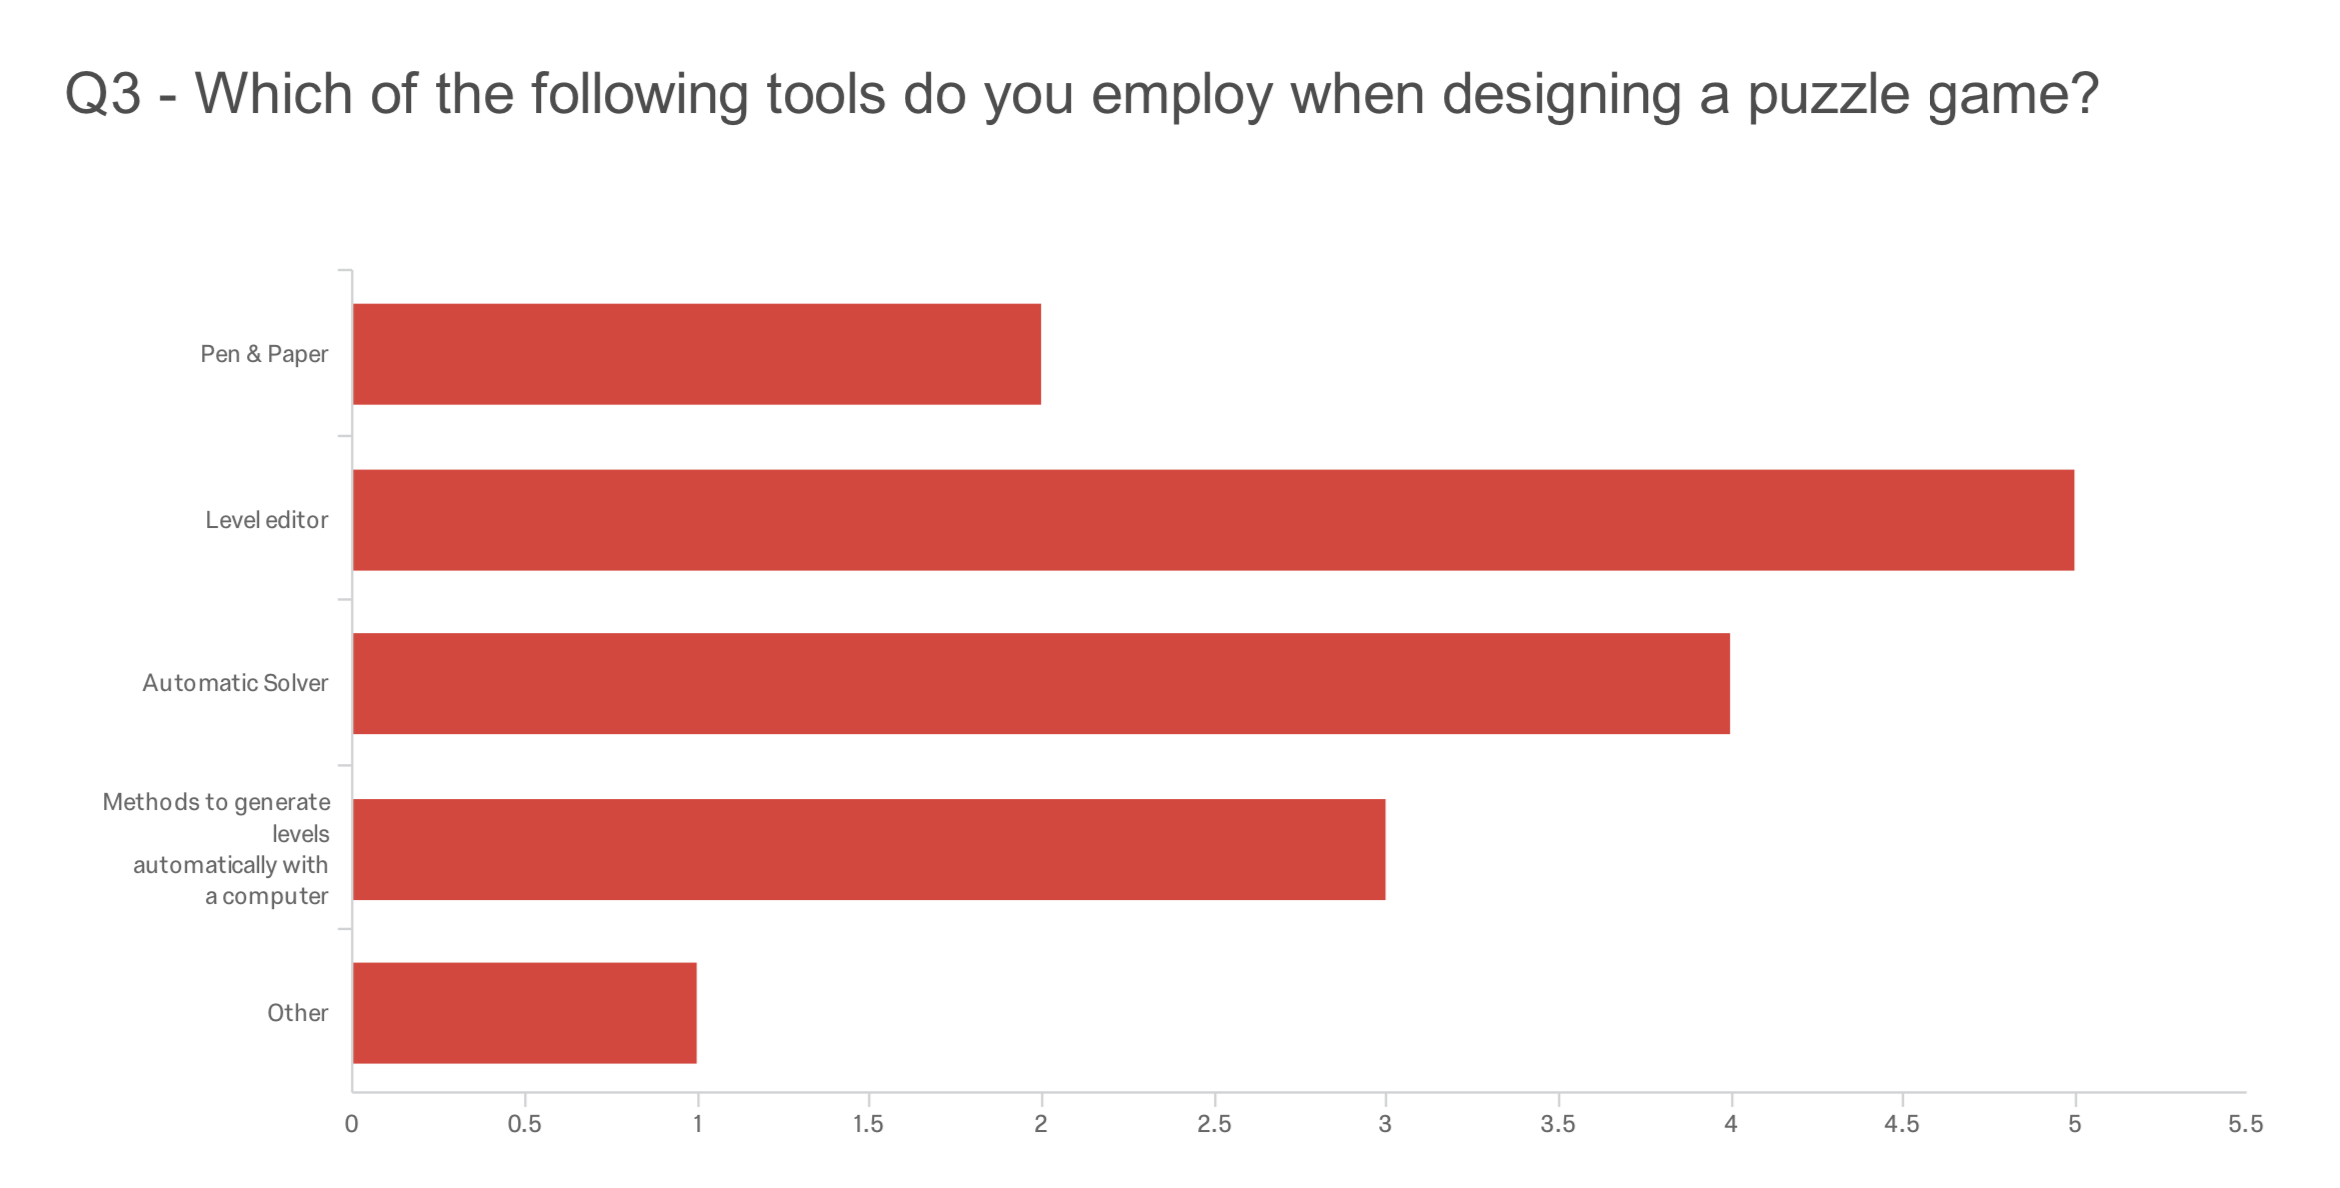
\includegraphics[width=1.0\linewidth]{figures/whichtoolsemployduringleveldesign.png}
    
    \caption[Needfinding]{Needfinding survey Q3 %
    \label{fig:needfindingq3}}
\end{figure}

% 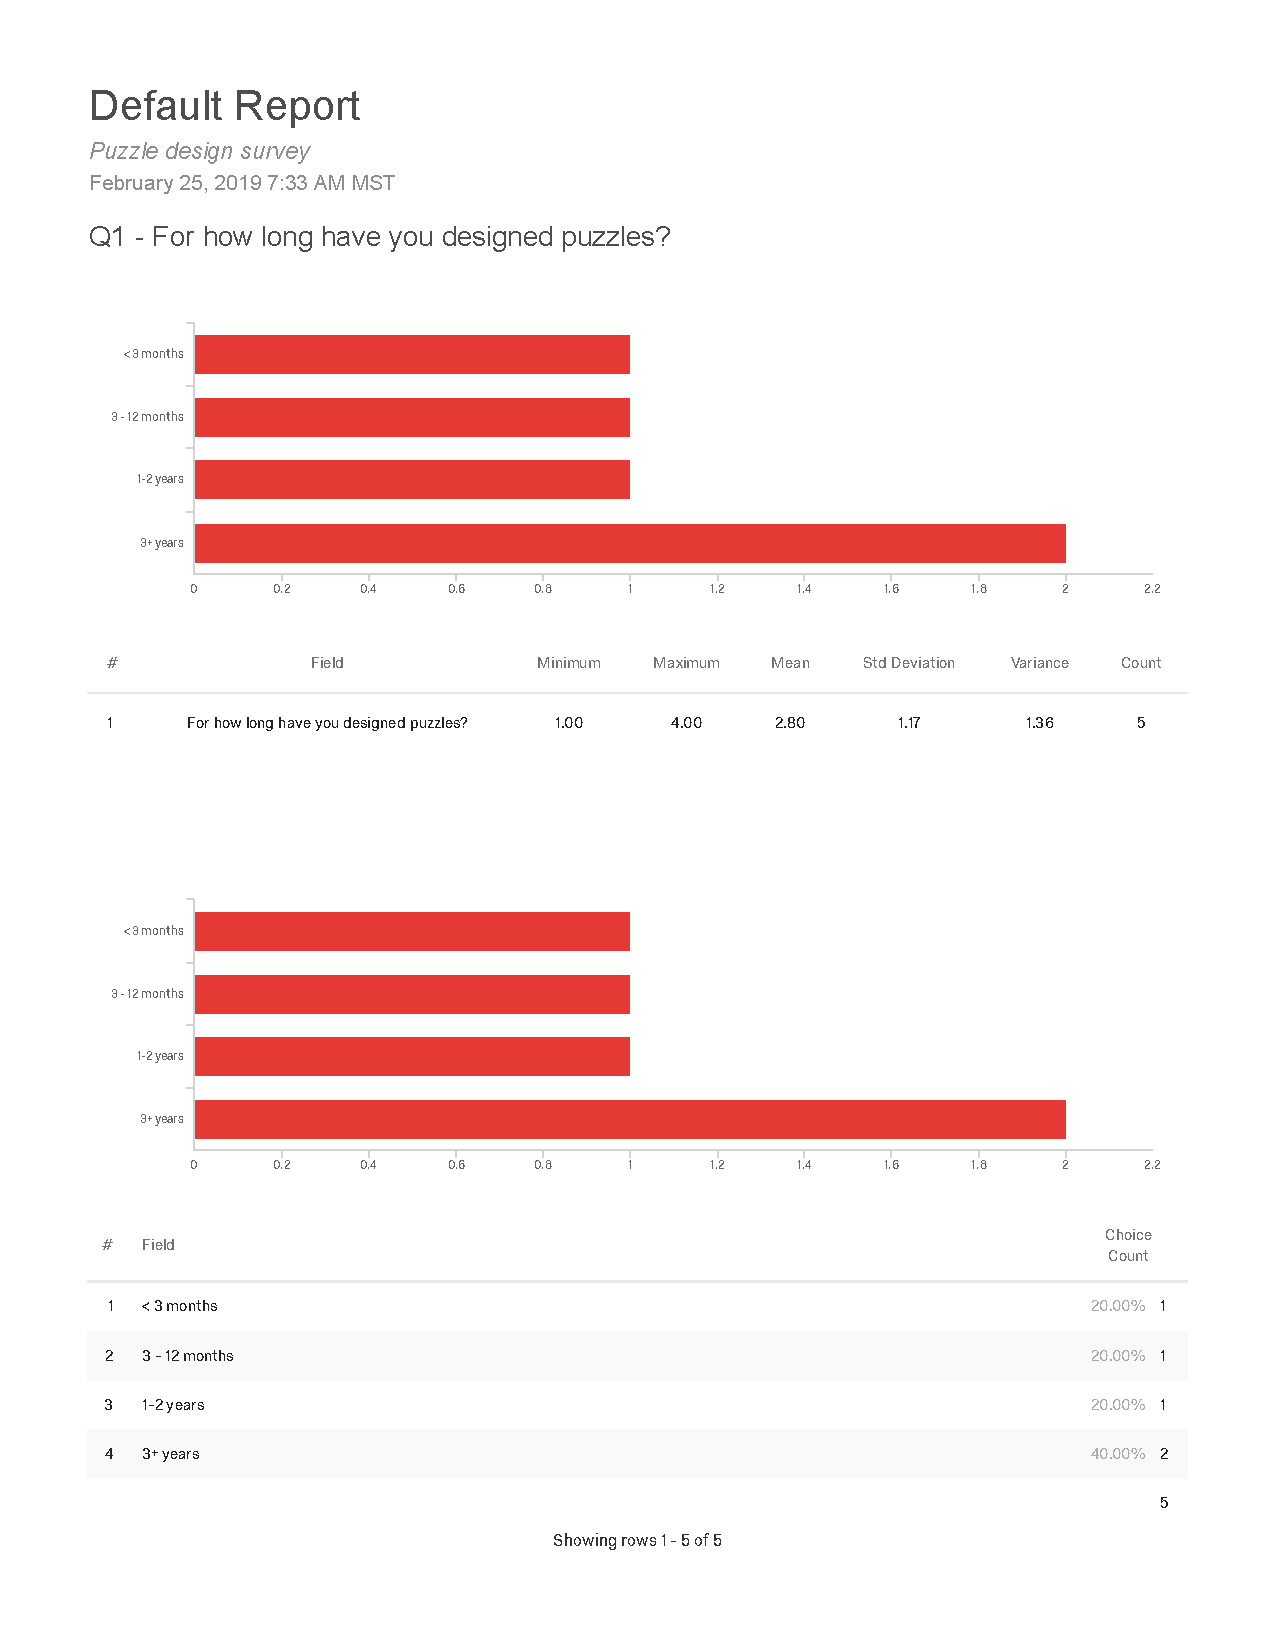
\includepdf[pages=-]{needfindingsurvey.pdf}

\section{PuzzleScript}

\begin{figure}
\centering
\begin{lstlisting}[language=PuzzleScript]
========
OBJECTS
========
Background
LIGHTGREEN

Target
DarkBlue

Wall
BROWN

Player
White

Crate
Orange

=======
LEGEND
=======
. = Background
# = Wall
P = Player
* = Crate
@ = Crate and Target
O = Target

=======
SOUNDS
=======
Crate MOVE 36772507

================
COLLISIONLAYERS
================
Background
Target
Player"Wall"Crate

======
RULES
======
[ >  Player | Crate ] -> [  >  Player | > Crate  ]

==============
WINCONDITIONS
==============
All Crate on Target

=======
LEVELS
=======
####..
#.O#..
#..###
#@P..#
#..*.#
#..###
####..
\end{lstlisting}
    \caption[Sokoban]{Example Sokoban implementation in PuzzleScript %
    \label{fig:sokobaninpuzzlescript}}
\end{figure}


\begin{figure}
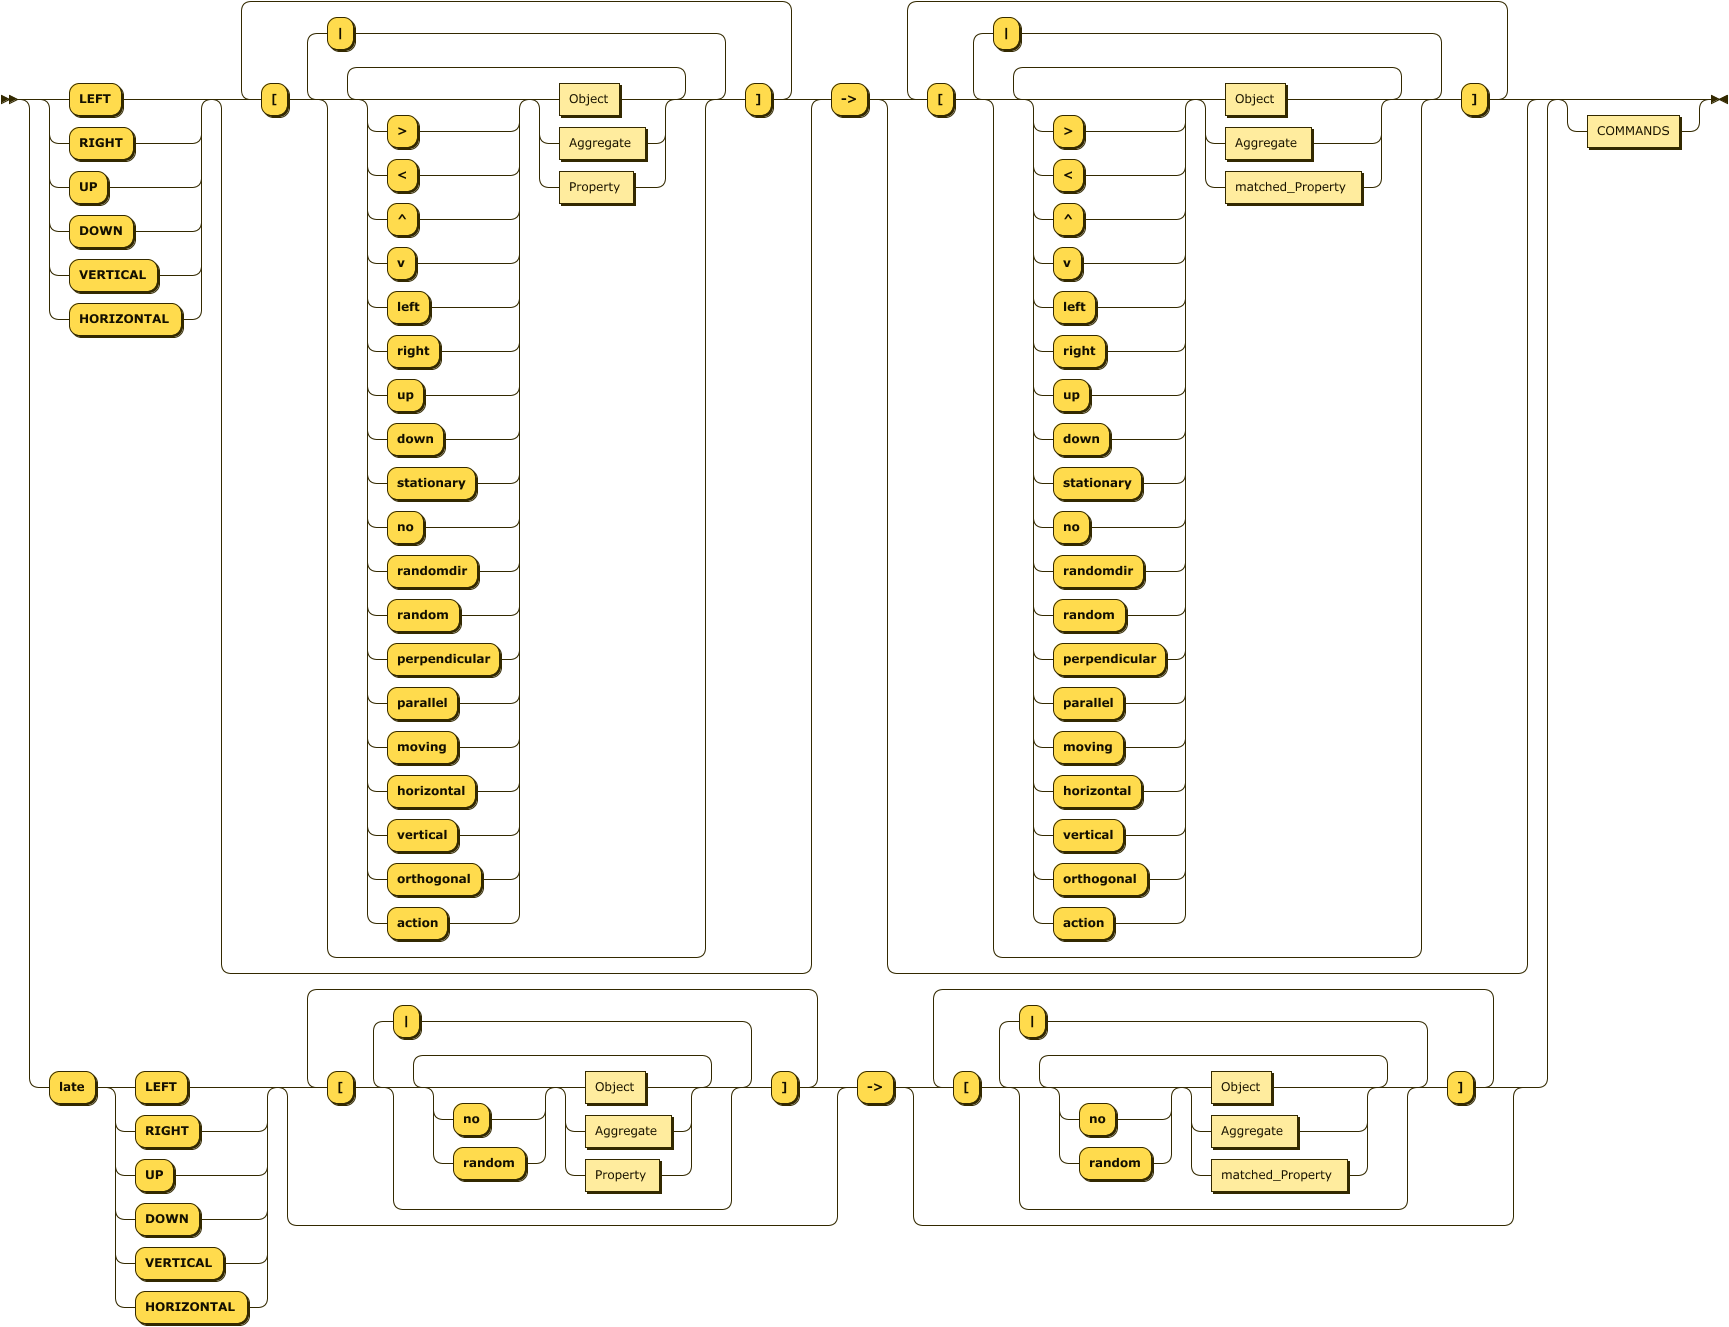
\includegraphics[width=1.0\linewidth]{figures/RULE_EXPANDED.png}
\caption[BNF Diagram]{ BNF Diagram for a PuzzleScript rule \textsuperscript{a)}\label{fig:puzzlescriptrulebnf}}
\small\textsuperscript{a)} Note that matched\_Property has to be a property that either appears only once on the left-hand side or a property that is exactly at the same location on the left-hand side. Whatever property it matches will be replaced on the right-hand side.
\end{figure}
\footnote{Note that matched\_Property has to be a property that either appears only once on the left-hand side or a property that is exactly at the same location where the property appears on the left-hand side. Whatever property it matches will be replaced on the right-hand side.}

\newpage


\section{User study}


\begin{figure}[!htbp]
\centering
\begin{minipage}[t]{0.2\textwidth}
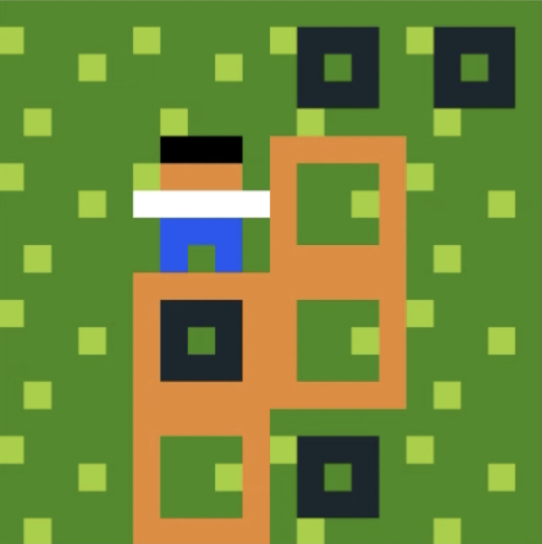
\includegraphics[width=\textwidth]{figures/finaldesign1_1.png} \hfill \\
\end{minipage}
$\:$
\begin{minipage}[t]{0.2\textwidth}
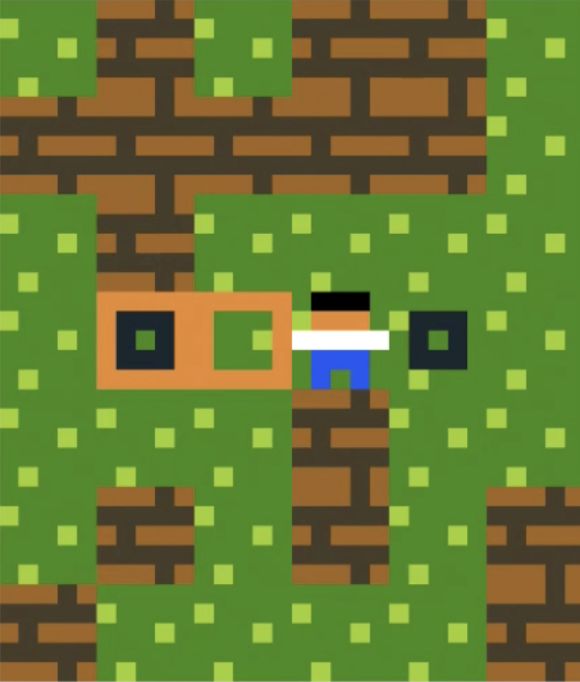
\includegraphics[width=\textwidth]{figures/finaldesign1_2.png} \hfill \\
\end{minipage}
$\:$
\begin{minipage}[t]{0.2\textwidth}
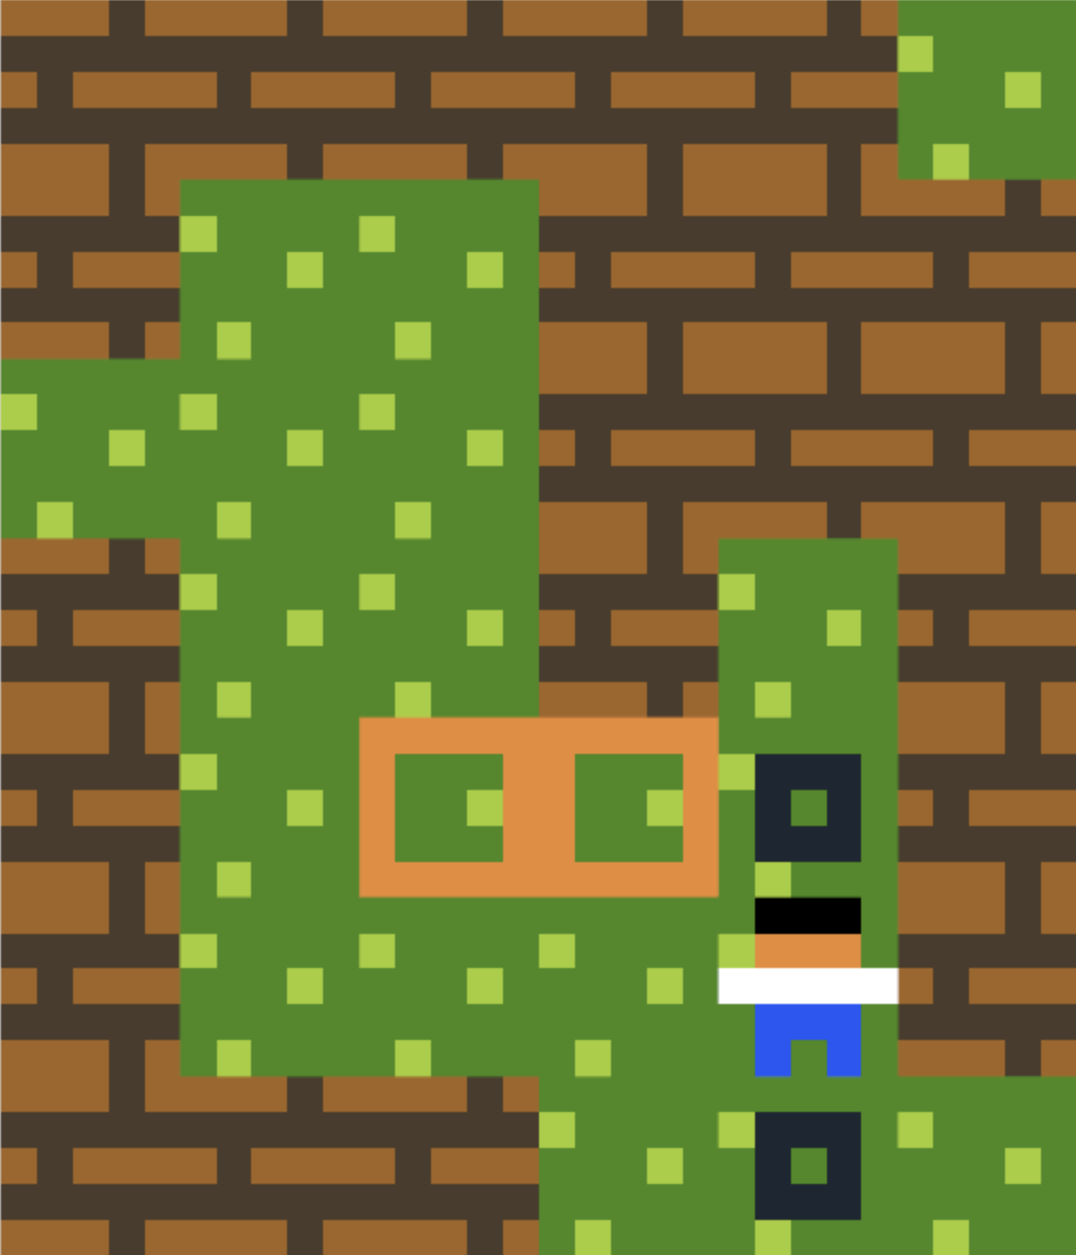
\includegraphics[width=\textwidth]{figures/finaldesign2_1.png} \hfill \\
\end{minipage}
$\:$
\begin{minipage}[t]{0.2\textwidth}
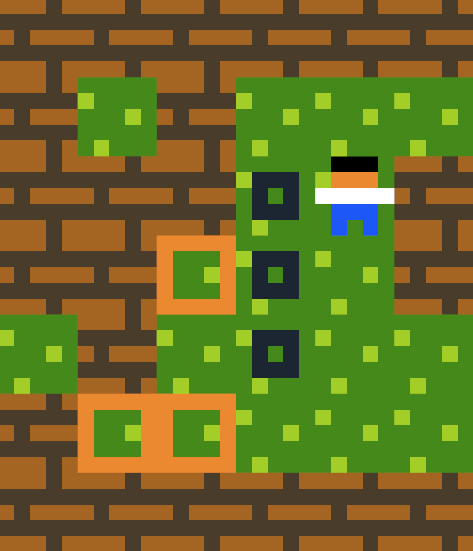
\includegraphics[width=\textwidth]{figures/finaldesign2_2.png} \hfill \\
\end{minipage}
$\:$
\begin{minipage}[t]{0.2\textwidth}
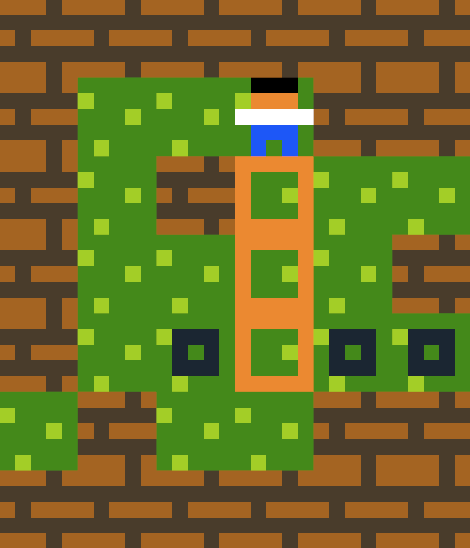
\includegraphics[width=\textwidth]{figures/finaldesign2_3.png} \hfill \\
\end{minipage}
$\:$
\begin{minipage}[t]{0.2\textwidth}
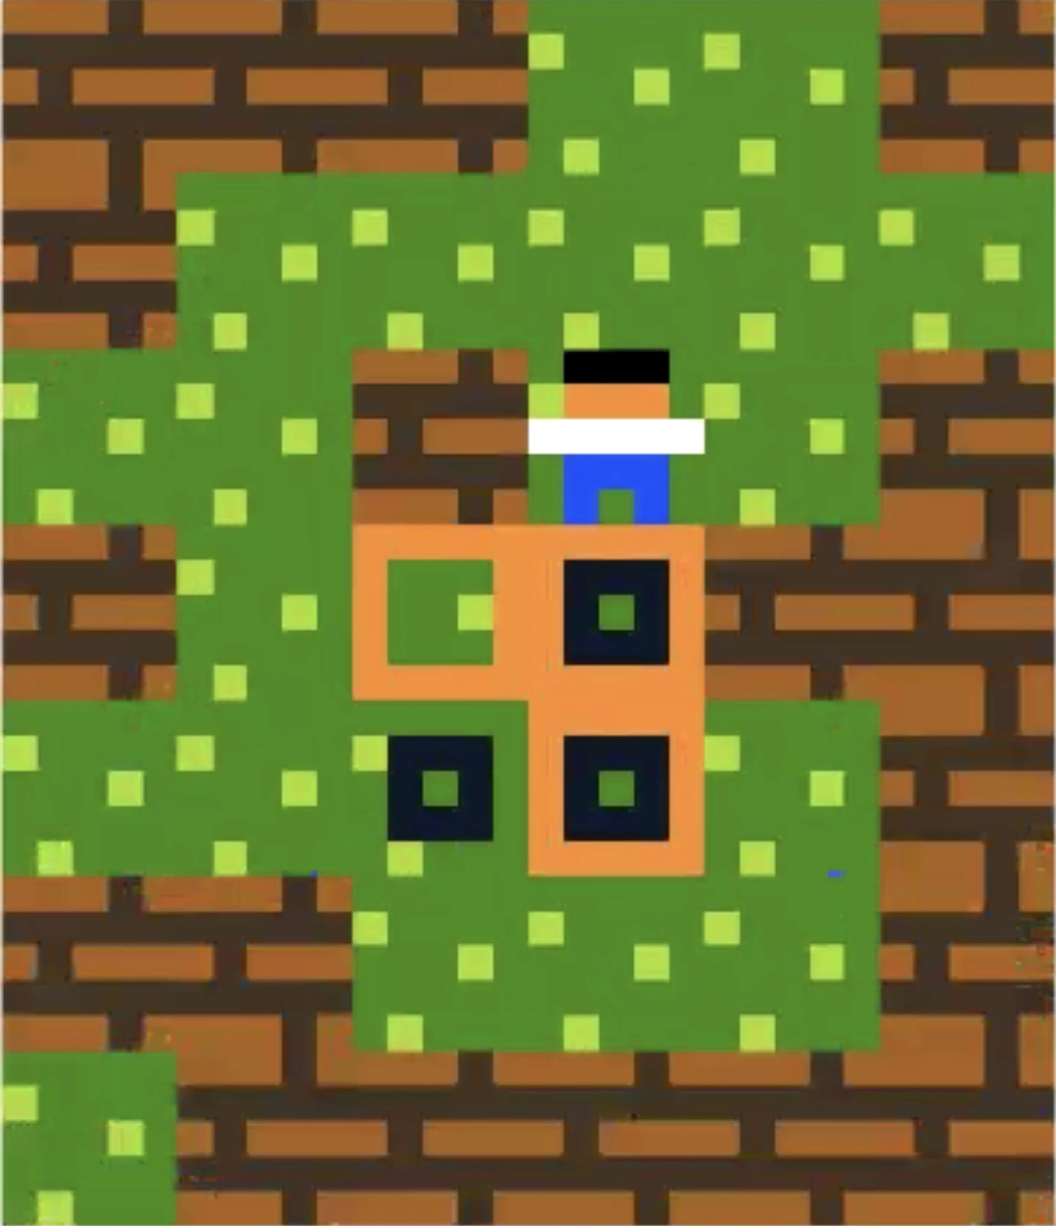
\includegraphics[width=\textwidth]{figures/finaldesign3_1.png} \hfill \\
\end{minipage}
$\:$
\begin{minipage}[t]{0.2\textwidth}
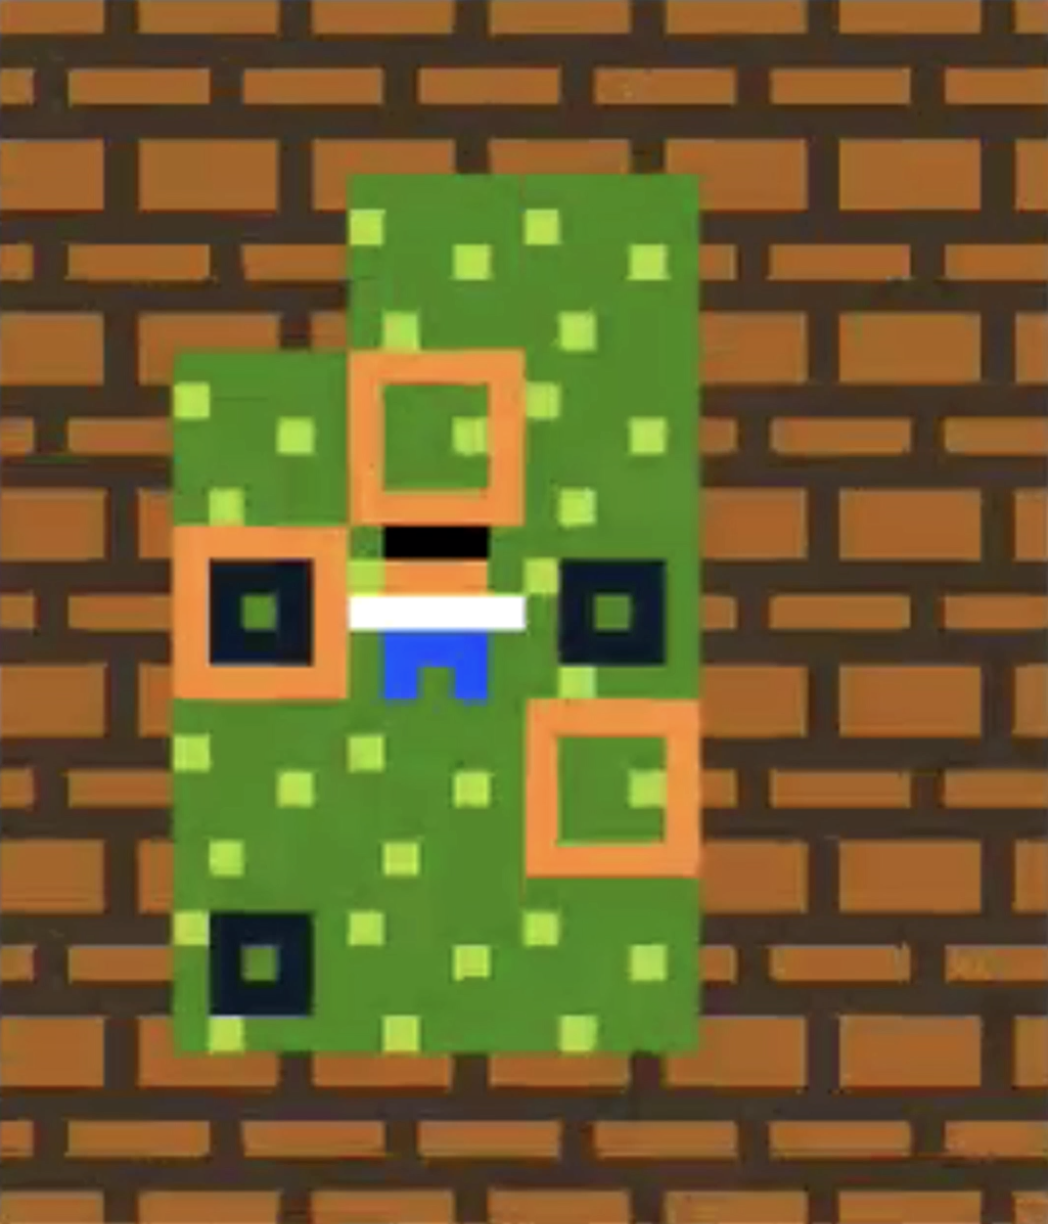
\includegraphics[width=\textwidth]{figures/finaldesign3_2.png} \hfill \\
\end{minipage}
$\:$
\begin{minipage}[t]{0.2\textwidth}
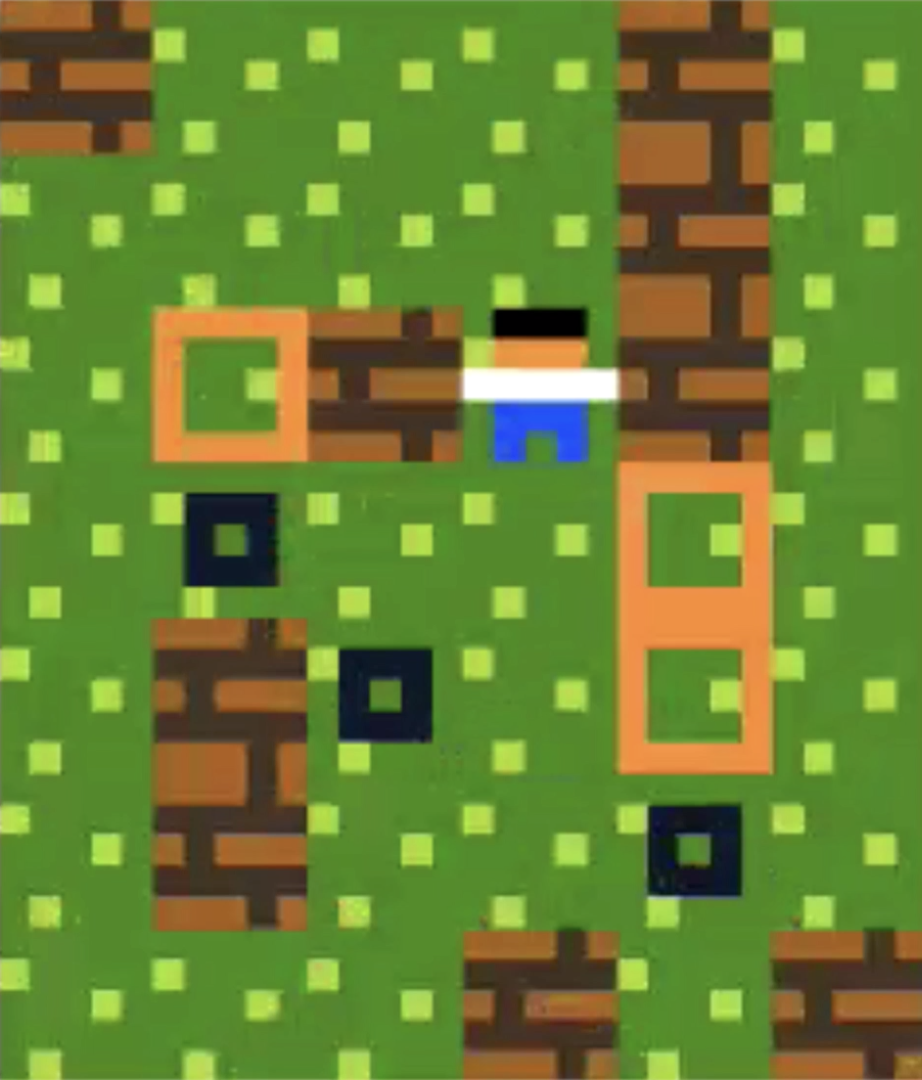
\includegraphics[width=\textwidth]{figures/finaldesign3_3.png} \hfill \\
\end{minipage}
$\:$
\begin{minipage}[t]{0.2\textwidth}
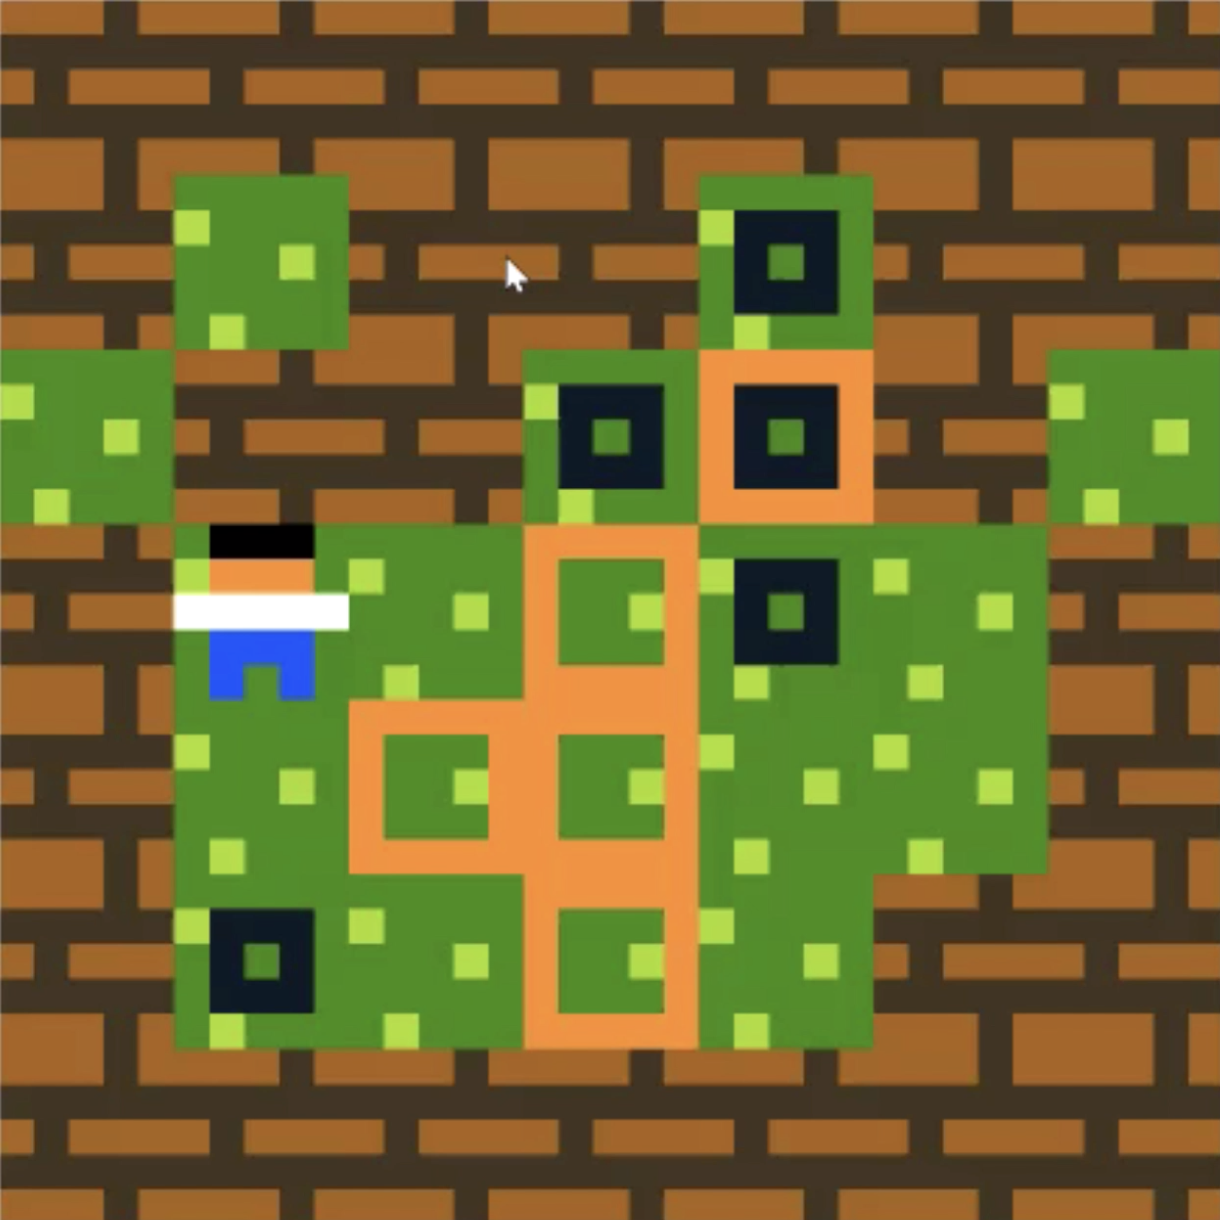
\includegraphics[width=\textwidth]{figures/finaldesign4_1.png} \hfill \\
\end{minipage}
$\:$
\begin{minipage}[t]{0.2\textwidth}
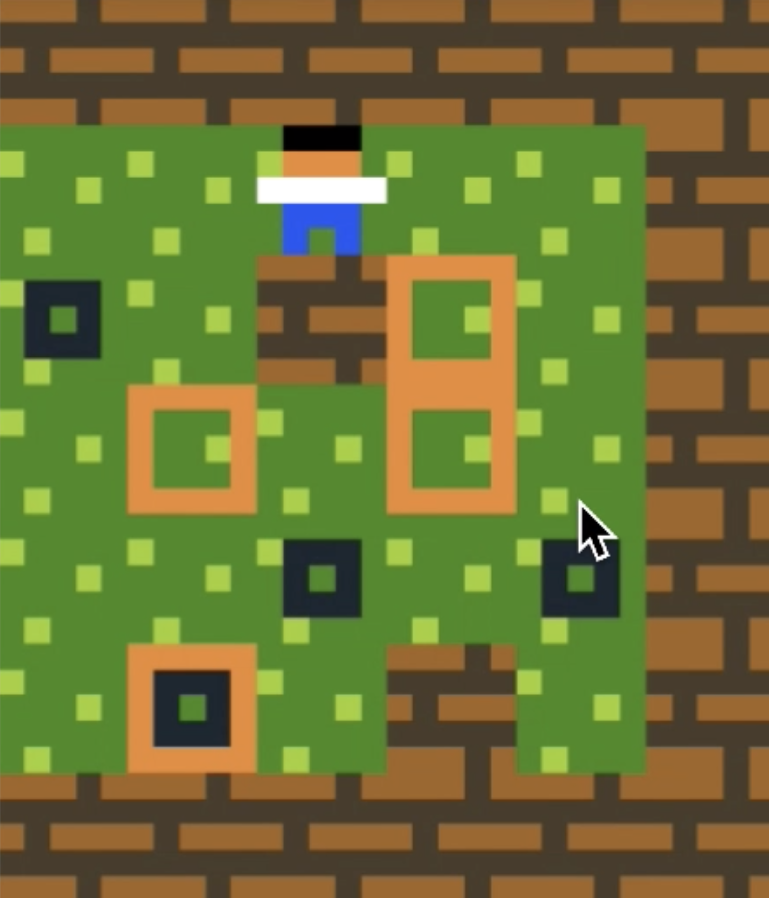
\includegraphics[width=\textwidth]{figures/finaldesign5_1.png} \hfill \\
\end{minipage}
$\:$
\begin{minipage}[t]{0.2\textwidth}
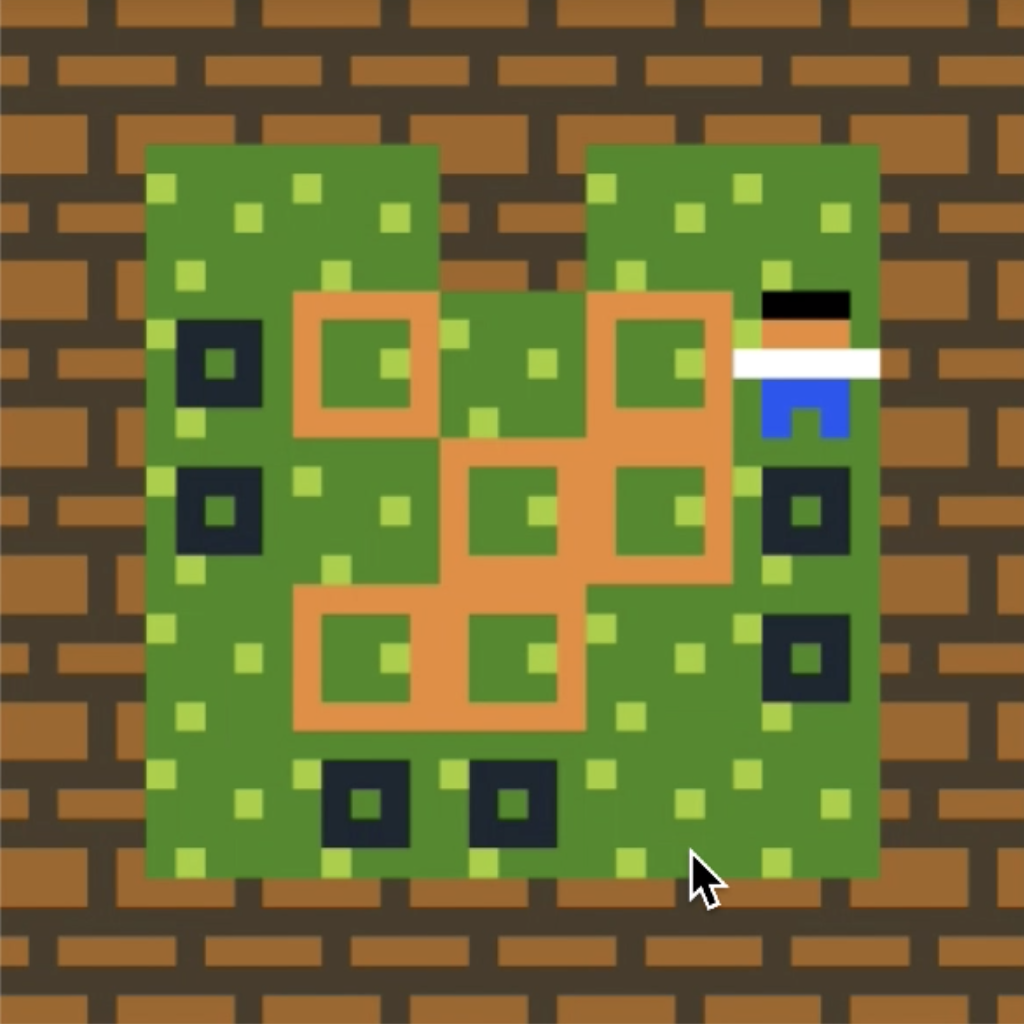
\includegraphics[width=\textwidth]{figures/finaldesign5_2.png} \hfill \\
\end{minipage}
$\:$
\begin{minipage}[t]{0.2\textwidth}
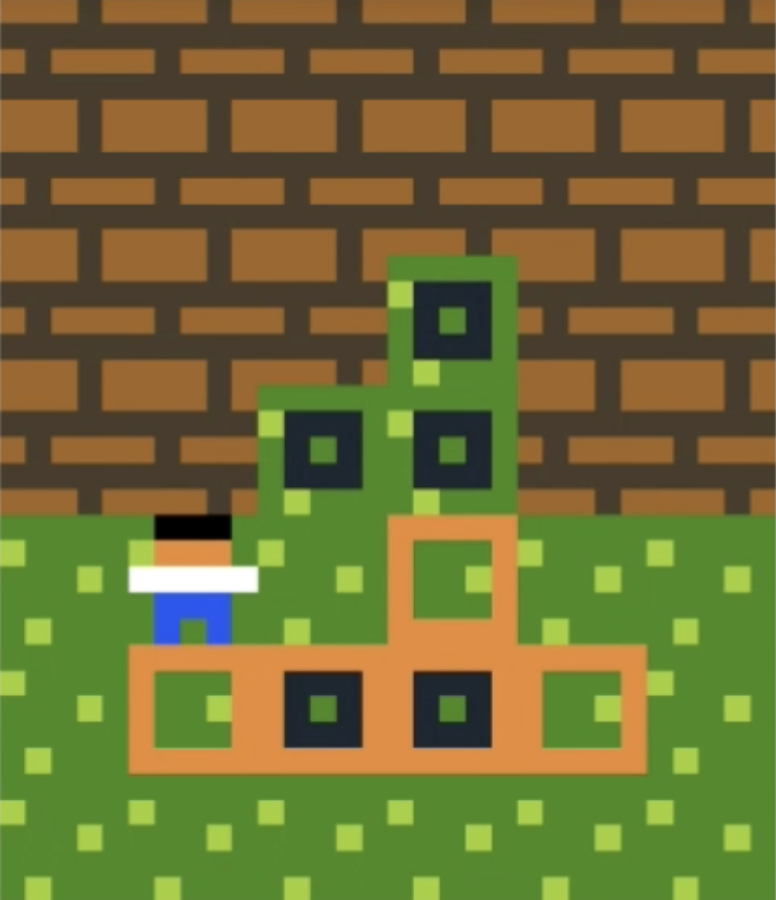
\includegraphics[width=\textwidth]{figures/finaldesign5_3.png} \hfill \\
\end{minipage}
$\:$
\begin{minipage}[t]{0.2\textwidth}
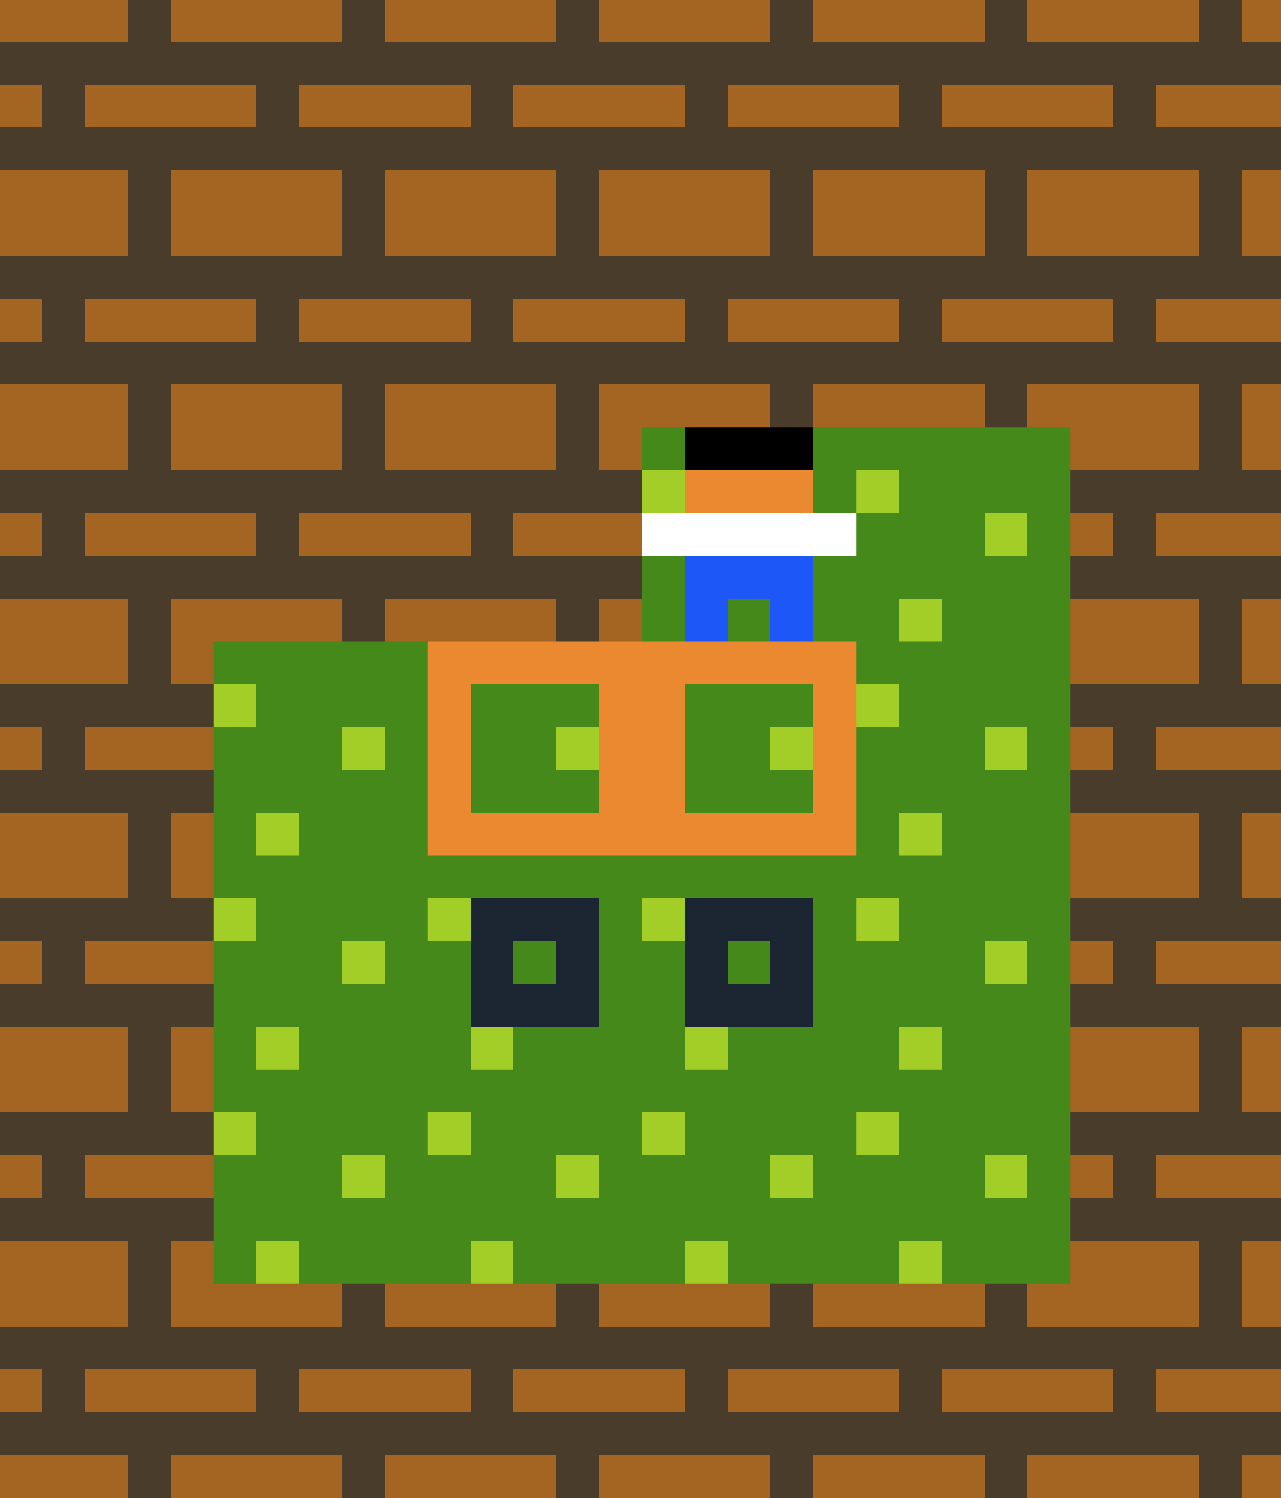
\includegraphics[width=\textwidth]{figures/finaldesign6_1.png} \hfill \\
\end{minipage}
$\:$
\begin{minipage}[t]{0.2\textwidth}
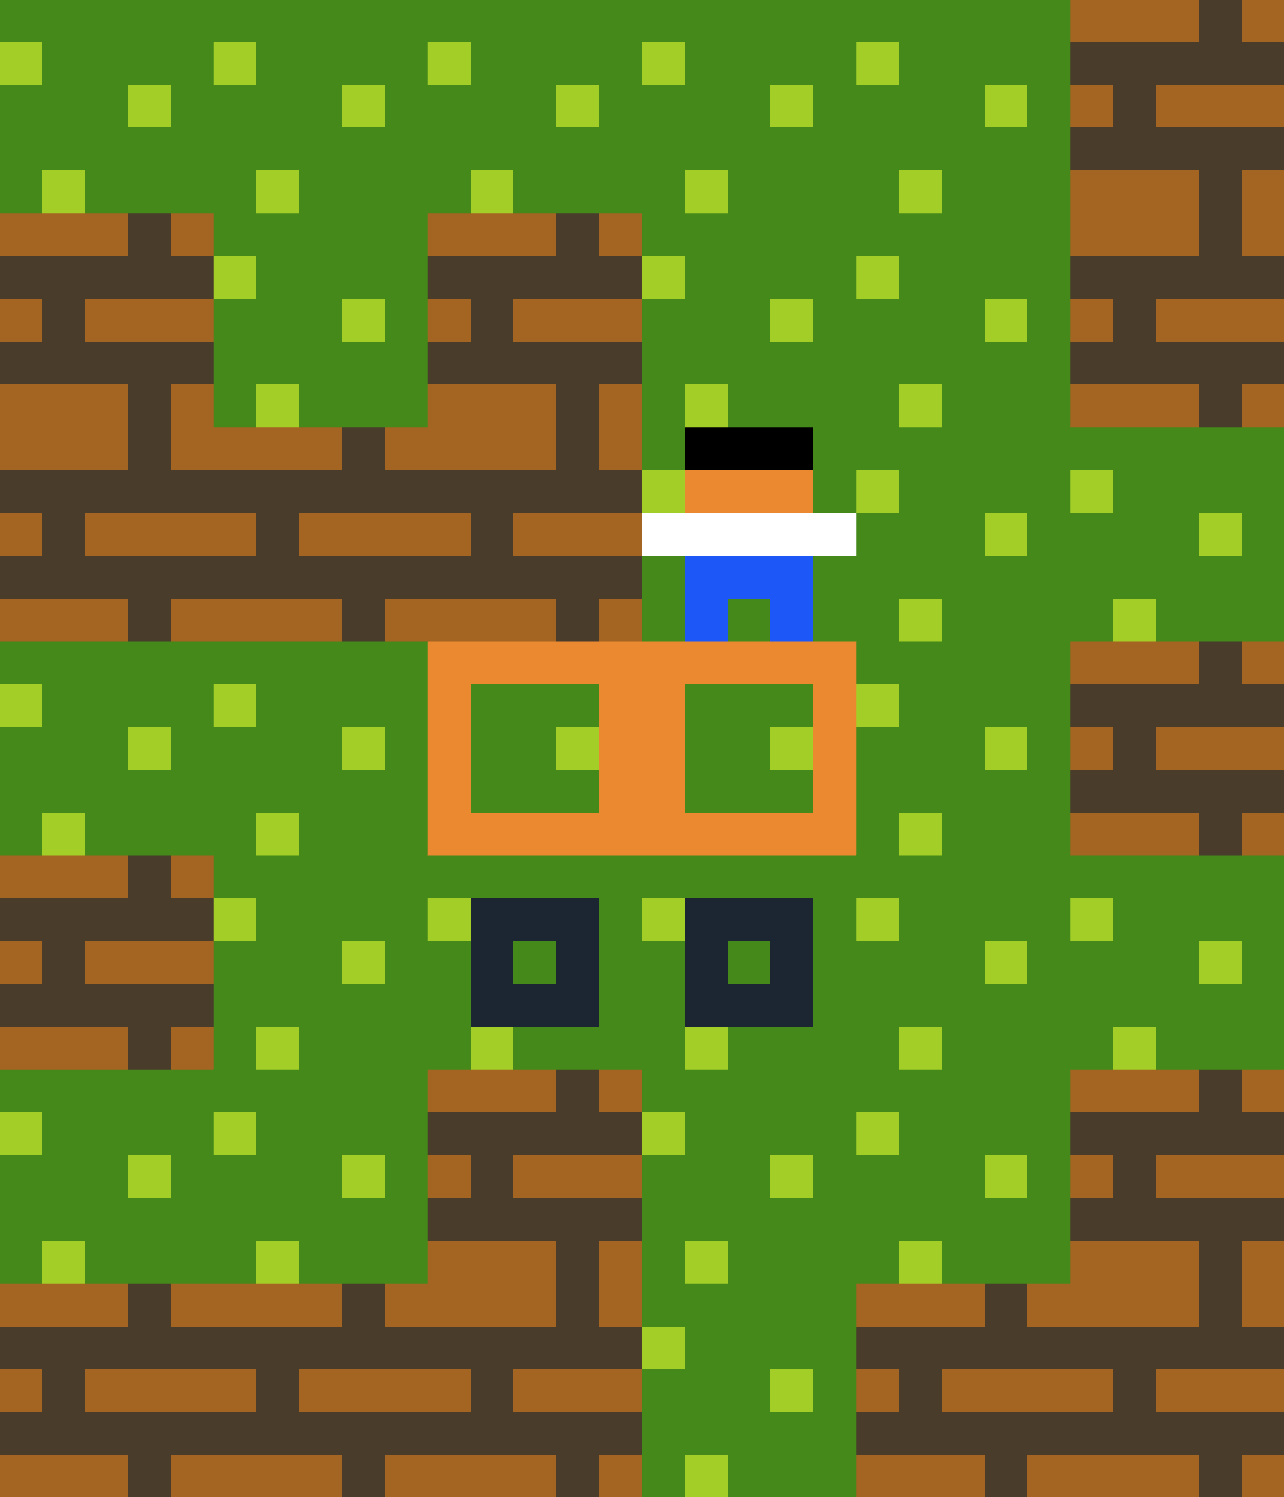
\includegraphics[width=\textwidth]{figures/finaldesign6_2.png} \hfill \\
\end{minipage}
$\:$
\begin{minipage}[t]{0.2\textwidth}
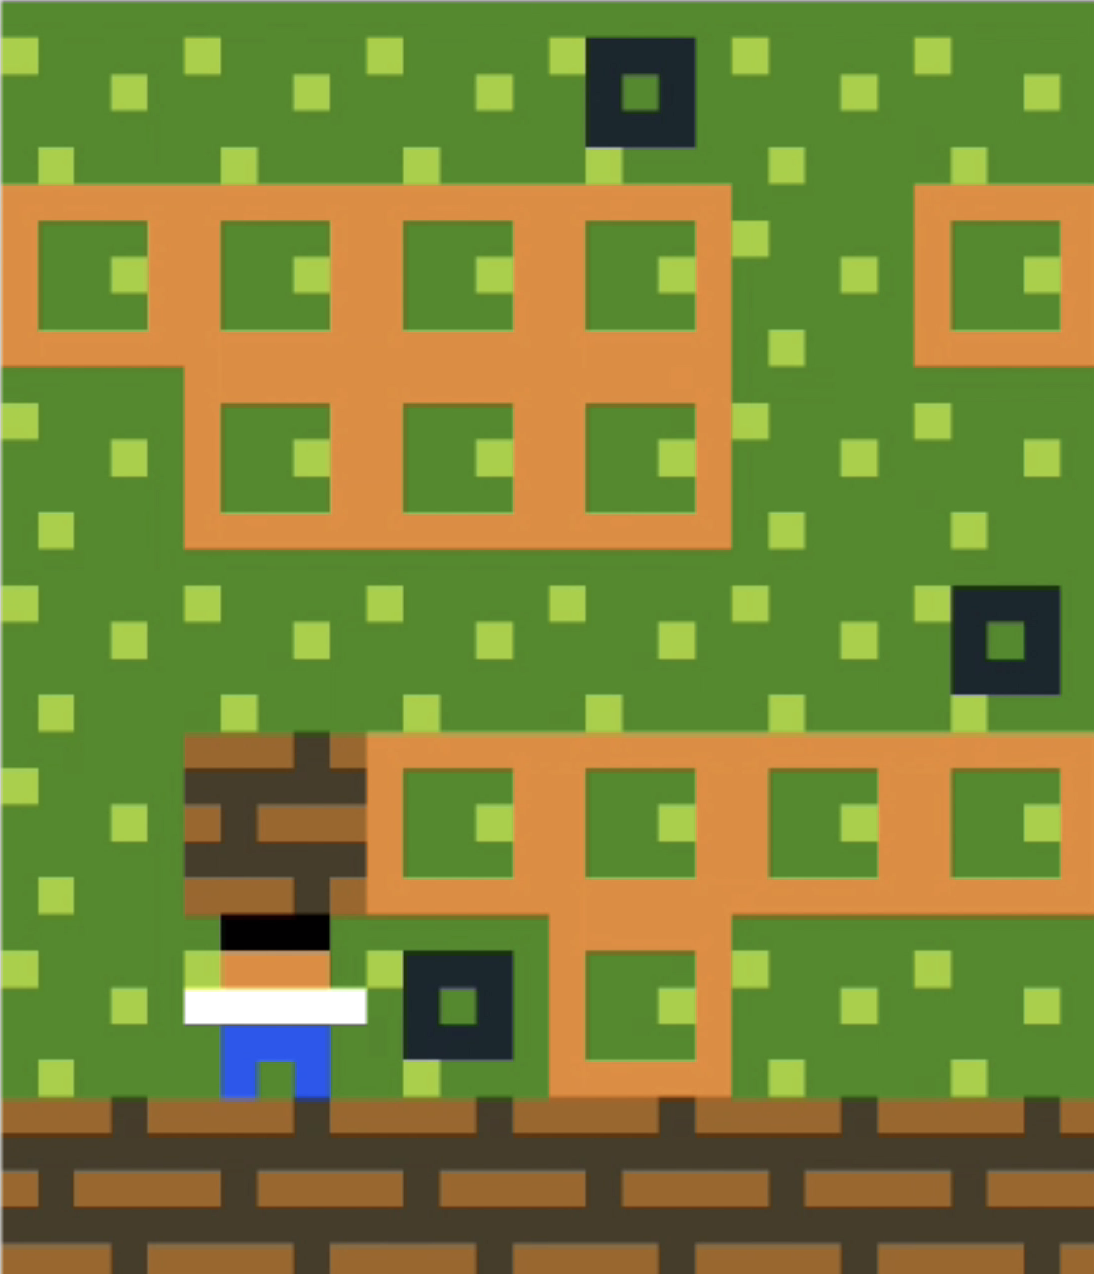
\includegraphics[width=\textwidth]{figures/finaldesign7_1.png} \hfill \\
\end{minipage}
$\:$
\begin{minipage}[t]{0.2\textwidth}
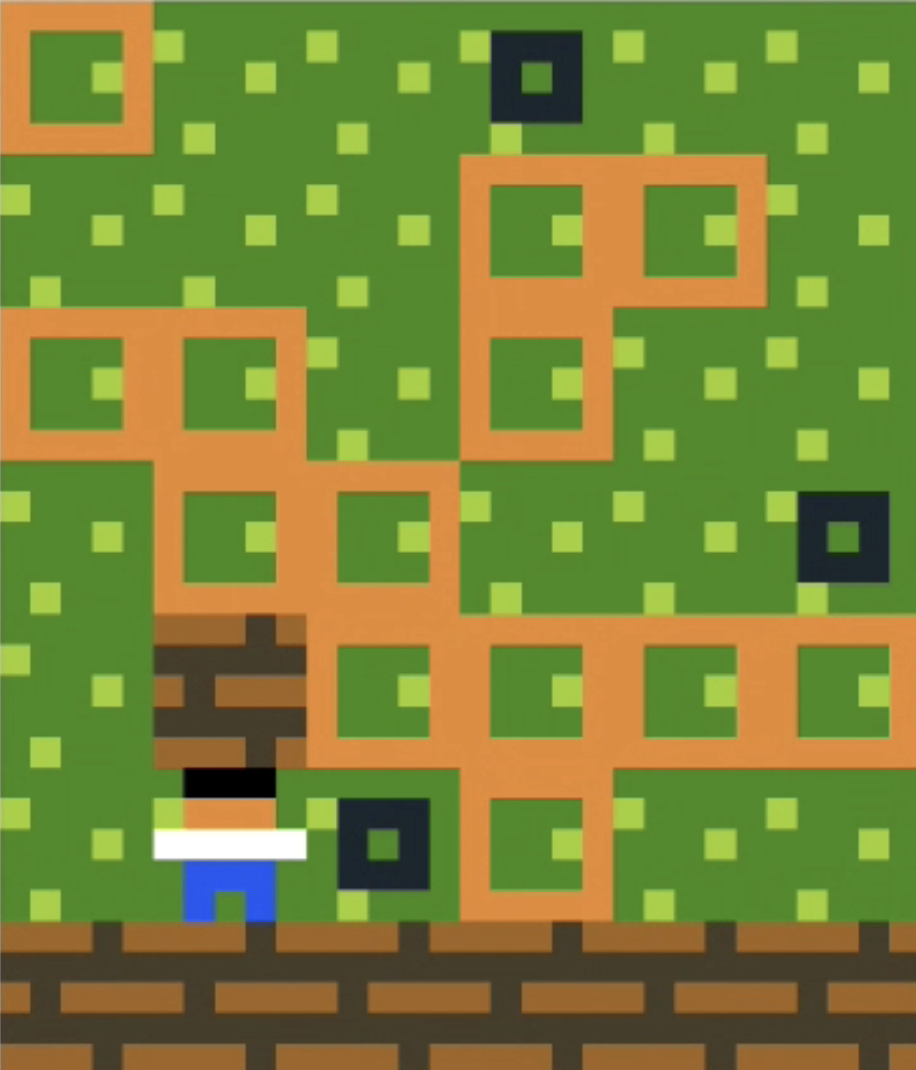
\includegraphics[width=\textwidth]{figures/finaldesign7_2.png} \hfill \\
\end{minipage}

\caption{All designs of the think-aloud study\label{fig:alldesigns}}
\end{figure}


\begin{sidewaystable}
\small
\begin{tabular}[t]{l||c|c|c|c|c|c|c}
\toprule
% Participant &  Stephen 1 & Marcos 2 & ThatScar 3 & 4 Minotalen & 5 Joel & 6 Max & Sam 7 \\
Participant &  1 & 2 & 3 & 4 & 5 & 6 & 7 \\
\midrule
Age & 34 & 46 & 20 & 25 & 30 & 27 & 28 \\
Gender & male & male & male & trans & male & male & male \\
Profession & game designer & \specialcell[t]{programmer \& \\ game designer} & junior programmer & design student & doctor & game designer & game designer \\
Puzzle Design Experience & 15 years & 8 years & 3 years on and off & 1 year, 3 games & 1 year, 200 hours & \specialcell[t]{2 days \\ 5 years (gd)} & 4 years \\
%How to design & Not quickly.  I've used a bazillion different techniques (on paper sometimes, in level editors with various levels of assistence, to fully autogenerated). &  &  . & forward design & fidn interesting geometry \\
\bottomrule
\end{tabular}
\caption{Demography of user study\label{tab:demography}}
\end{sidewaystable}


\section{Structured interview questions\label{apx:interview}}

This is a compiled list of the most interesting answers to the interview questions:


\textbf{Tell me about your experience with the editor.}

\textit{\say{In broad terms it does some cool things. Bunch of usability suggestions. I have to figure out more use cases.} -- Participant 1}

\textit{\say{Overall it's a very interesting project. Some quirks of the interface are to be solved but I hope you can expand it and make it more powerful.} -- Participant 2}

\textit{\say{The editor was fun to use, but oftentimes I found it was lacking visual feedback of the ongoing generation process.} -- Participant 4}

\textbf{How was this design process different from your usual practice?}

\textit{\say{Designing with a level generator gives the advantage of encountering new object 'constellations' that are sometimes unintuitive and difficult to solve.} -- Participant 4}

\textit{\say{Faster, felt like communication, not trivial.} -- Participant 6}

\textit{\say{The loop of mutating/trying/repeat is very appealing, reminiscent to genetic art generators. Usually I make a loop of generating/curating/repeat for my games, perhaps this type of tool can insert a very useful step with the mutator.} -- Participant 2}

\textbf{How satisfied are you with the design(s)?}

\textit{\say{Some of the levels I found are very surprising and pleasing.} -- Participant 2}

\textit{\say{I wasn't happy with the designs (of the Sokoban levels) but attribute that mainly to my error, could have used a more interesting generation algorithm and level base. Sokoban levels have been generated for ages, so my levels were probably not original. Maybe going with a different base game (block pulling maybe?) would have resulted in more originality.} -- Participant 4}

\textit{\say{The levels are already quite neat! I'd say about 20\% were really interesting.} -- Participant 6}

\textit{\say{Not particularly.} -- Participant 5}

\textbf{How original do you think are the levels?}

\textit{\say{Not really. There should be more curated suggestion levels.} -- Participant 6}

\textbf{Did the functionalities hinder you to do anything and if yes what was it?}

\textit{\say{I did more than I imagined I could with the tool.} -- Participant 3}

\textit{\say{Some elements of the interface are difficult to understand at first, and some others are difficult to use, like the text editor.} -- Participant 1}

\textit{\say{The editor had most of the functionality that it needs, some 'quality of level' improvements would be required to tie it all together though. Not being able to alter level size from within the editor was annoying, also the Transform text box clearing on tab switch was a hindrance. Not being able to alter level size from within the editor was annoying, also the Transform text box clearing on tab switch was a hindrance.} -- Participant 4}

\textit{\say{I was able to do more in a short amount of time and check more things than I would usually.} -- Participant 6}

\textbf{Can you tell me how you experienced the interaction with the editor?}

\textit{\say{I used mainly the mouse, and some of the suggested shortcuts. I did not try to use the text editor very much.} -- Participant 2}

\textit{\say{Without the verbal confirmation that the generator is working I'd have believed it was not generating and kept restarting the process. Otherwise it was mostly fine.} -- Participant 4}

\textit{\say{It felt like a communication with the exception of the things I controlled.} -- Participant 6} (Note: This participant only used the suggested buttons and did not implement his own transformation rules).

\textit{\say{Watching numbers go up and gradually in the transformer and if it's too slow i'll change the transforms and fiddle with the level size. The polishing at the end I do by hand.}  -- Participant 1}

\textbf{How useful were the suggestions by the system? How did they help you?}

\textit{\say{The mutations were generally chaotic, but some of them were surprising, apparently impossible to solve, hence very fun to solve.} -- Participant 2}

\textit{\say{The level suggestions were as useful as the generation rules I fed into the system. The suggestions can be helpful for coming up with own design ideas.} -- Participant 4}

\textbf{Did you think that the system pointed you in different directions than you intended?}

\textit{\say{If the purpose of the system is generating new ideas, then new ideas would be an intended direction, so no.} -- Participant 4}

\textit{\say{I was just trying to figure out what the tool can and cannot do.} -- Participant 1}

\textit{\say{Not much, only worked well on smaller sized levels.} -- Participant 5}

\textbf{In your view, how did the system make the suggestions?}

\textit{\say{I suspect the system uses digital mutation operations that modify the current element of the levels, and tries to solve the new levels, discarding unsolvable/trivial ones.} -- Participant 2}

\textit{\say{It made the suggestions based on the results of my transformation rules, a solver and a complexity rating algorithm.} -- Participant 4}

\textbf{Can you reflect on how your behaviour impacted the suggestions of the system?}

\textit{\say{I feel that the selection of levels from me reinforces the kind of variations the system makes later.} -- Participant 2}

\textit{\say{The transformation rules directly impact what levels are generated, the solvable subset of those gets rated by complexity, the four highest-razed levels get presented to me, so the impact of the rules is indirect.} -- Participant 4}

\textit{\say{Well I kind of knew what it did after you explained it so it just did what I wanted it to do.} -- Participant 6}

\textit{\say{The modify and leave buttons impacted it.} -- Participant 3} 

\textbf{How much did you feel the system understood your aim?}

\textit{\say{I feel like in its current state the system does not use all the feedback loops it could use.} -- Participant 2}

\textit{\say{The system has the aim of creating complex levels from a set of rules. Formulating intentions would happen by setting rules and base level but the system would not 'understand', just process.} -- Participant 4}

\textit{\say{Pretty well.} -- Participant 1} % I'm learning what the system can do to get an idea how it works

\textit{\say{It didn't really \say{understand} it since it's just a tool.} -- Participant 3}

\textit{\say{It is not intelligent, it just did what I told it to do and it was a useful tool.} -- Participant 6}

\textbf{How would you characterise the tool within the design process?}

\textit{\say{As an integral part, like a canvas where experiment within the level space.} -- Participant 2}

\textit{\say{Perhaps useful for coming up with variations and unintuitive level designs.} -- Participant 4}

\textit{\say{The role of saving levels, playing them, checking if they are solvable and finding their solutions if so. Additionally, it brought me ideas and did its job quite well.} -- Participant 6}

\textit{\say{I don't have a loop of iterative design, I'm just looking for a good starting point.
The suggestions are nice and interesting.} -- Participant 1}

\textbf{How well did the scores for the difficulty of the level match your estimation?}

\textit{\say{Good enough to be useful, but somewhat uneven. I believe the system could integrate more evaluation criteria to make the estimation more exact.} -- Participant 2}

\textit{\say{Difficulty rating did not align with my perception of difficulty, but I've not yet explored enough to be sure.} -- Participant 4}

\textit{\say{I did not look at the difficulty scores, just at the curated levels.} -- Participant 6}

\textit{\say{Pretty accurate, there seems to be a threshold starting from which the levels get interesting, at least that's how it feels like qualitatively.} -- Participant 1}

\textbf{Did a suggestion inspire you without you clicking on it?}

\textit{\say{Yea, exactly what happened in the end.} -- Participant 3}

\textit{\say{Yes, especially as a level of confidence so I was sure that the current design was pretty solid when the suggestions seemed worse.} -- Participant 6}

\textit{\say{No, but could happen. Looking at them and trying to solve them in the head is slower than just clicking on them to try it out.} -- Participant 1}

Note: The people who said no were simply adapt at quickly trying out a suggestion and popping back to the old design.

\textbf{Would you use such a system in your work practice and when? 
If Yes: What for in specific; If No: What needs to be changed?}

\textit{\say{I would use it to find new levels for my games, but also to inspire my level generators with some kind of variations I usually don't explore because lack of real time visualisation.} -- Participant 2}

\textit{\say{Yes, for creating level states that I hadn't encountered before, then using those as inspiration.} -- Participant 4}

\textit{\say{Not for the game I'm currently working on but if I design a puzzle game in the future again sure.} -- Participant 6}

\textit{\say{Yea, for certain particular games. Also for super compact levels on any kind of puzzle game.} -- Participant 1}

\textbf{Where do you see the potential of such systems and where the limitation?}

\textit{\say{There is great potential to explore rule variation in addition to level variation. Limitations are, like always, memory and cpu usage when using mutators and solvers not tuned to specific rules.} -- Participant 2}

\textit{\say{Potential for creating unintuitive and thus hard to solve levels. Potential for improving handmade levels. Limitation in  complexity heuristics and level size (since computation effort increases exponentially)} -- Participant 3}

\textit{\say{Potential is to create low effort levels and it allows you to constrain your creativity. There's a kind of Google effect where I stop thinking about solvability. Probably if you've been designing puzzles for a specific game for a long period of time the tool probably won't help much anymore, so it's more useful in the prototype phase. The limits are the language of PuzzleScript and the language of the transformer.} -- Participant 4}

\textit{\say{Performance limitations. Level size, \# of rules, people making bad levels with it, people making levels that aren't fun. I'm always going to try to make small levels with it.} -- Participant 1}

\textit{\say{The limitations are [the systems] judging abilities.} -- Participant 3}

\textbf{Do you have any thoughts you would like to add?}

\textit{\say{I hope more kind of games are added later to the system (3D and/or continuous-like rules).
This project is very promising, I cannot wait to try the next version, and possibly contribute to it.} -- Participant 2}

